\documentclass[12pt,a4paper]{scrartcl}
\usepackage[protrusion=true,expansion=true]{microtype}
\linespread{1.3}

\usepackage{float}
\usepackage{amssymb}
\usepackage{caption}
\usepackage[utf8]{inputenc}
\usepackage[T1]{fontenc}
\usepackage{graphicx}
\usepackage[bookmarks=true,hidelinks=true,breaklinks=true]{hyperref}
\usepackage{mathptmx}
\usepackage{cleveref}
\usepackage{enumitem}
\usepackage{minted}
\usepackage[backend=biber,natbib=true]{biblatex}
\usepackage[scaled=.92]{helvet}
\bibliography{references.bib}

\begin{document}
\title{Der Transparente Mensch: Die unvermeidliche Preisgabe von Metadaten }
\author{Arne Beer, MN 6489196, University of Hamburg}
\date{20.08.2019}

\maketitle


\section{Abstract}

Metadaten spielen eine bedeutende Rolle in der Welt der Datenanalyse.
Simple Informationen über einen Menschen, wie zum Beispiel der Standort verknüpft mit Zeitpunkten, verschiedene Aktivitäten oder Vorlieben, liefern enormes Potential, um diesen zu analysieren und kategorisieren.
In vielen Fällen wird aktives Sammeln von Daten, Data Mining und Big Data Analysis betrieben und Plattformen wie Facebook, haben sich voll diesem Ziel verschrieben.

Metadaten sind jedoch tückisch und befinden sich an viel mehr Orten als man vielleicht auf den ersten Blick vermutet.

Dieses Paper wird sich speziell mit der Intransparenz in Bezug auf die Freigabe von Metadaten bei bestimmten Tools auseinandersetzen, welche eigentlich nicht für diesen Zweck vorgesehen sind.
Speziell betrachten wir in diesem Falle das Tool \emph{Git}, welches hauptsächlich zur Versionskontrolle von Quellcode in Informationstechnischen Projekten verwendet wird.
Zudem wird die populäre Website \emph{GitHub} betrachtet, welche als Open-Source Plattform dient, auf der jeder Entwickler seine Projekte öffentlich zur Verfügung stellen kann.

\newpage

\section{Einleitung}
Das Ziel dieser Arbeit ist, die Notwendigkeit von Datenerfassung zu betrachten.
In einigen Umfeldern, speziell im Informationstechnischem Bereich, ist die Erfassung von Metadaten unvermeidlich und teilweise unabdingbar.
Daten werden zur Analyse von technischen Prozessen benötigt oder um z.B. die Verantwortlichkeit eines Entwicklers für eine bestimmte Änderung an einem System festzuhalten.

Leider lassen sich aus simplen Metadaten jedoch häufig mithilfe von Data Mining Techniken mehr Informationen als auf den ersten Blick ersichtlich.
Hierbei kann es dazu kommen, dass durch simple Hilfsmittel, welche lediglich die Produktivität und Benutzbarkeit eines Werkzeugs verbessern sollen, private Informationen über den Nutzbar nach außen hin ersichtlich werden.
Falls diese Daten nun zusätzlich öffentlich einsehbar sind, können diese von einer nicht kontrollierten Instanz benutzt werden.

Aus diesen Umständen entsteht ein Dilemma, welches aus dem Konflikt zwischen der Notwendigkeit Daten zu erheben und zu veröffentlichen und der unmöglichen Kontrolle über die Verbreitung dieser Daten besteht.
Im Folgenden wird dieses Problem in Bezug auf Privatheit und Transparenz am Beispiel der professionellen Open-Source Community und dem Tool Git näher betrachtet.

\section{Git und Github}
Diese Arbeit erläutert die vorliegende Problematik am Beispiel des Tools \emph{Git} und der Plattform \emph{GitHub}.
Hierzu werden im Folgenden die beiden Technologien vorgestellt, wichtige Aspekte erörtert und zusammengefasst.


\subsection{Git}
Git ist ein heutzutage als Standard angesehenes Werkzeug zum Entwickeln von Projekten im Informationstechnischen Sektor.
Beinahe jedes Projekt mit Quellcode besitzt eine Art von Version Control System (VCS), und in den meisten Fällen wird diese Rolle von \emph{Git} eingenommen.
Ein VCS ist ein Hilfsmittel, welches es erlaubt den Quellcode zu versionieren, also zu bestimmten Zeitpunkten eine Version des momentanen Standes des Projekts festzuhalten.
Ein Projekt, welches von Git verwaltet wird, wird im Fachjargon ein \emph{Repository} genannt.

Durch diese Versionierung, ist es den Entwicklern des Projekts möglich schnell zwischen verschiedenen Versionen hin und her zu wechseln.
Sollte also zum Beispiel ein neues Feature einer Software fehlerhaft sein und nicht funktionieren, kann mithilfe eines Befehls ohne weiteren Aufwand zu der vorherigen stabilen Version des Projektes gewechselt werden.
Eine solche Version wird in Git als \emph{Commit} bezeichnet.
Ein \emph{Commit} kann nun wiederum auf einen oder mehrere andere \emph{Commits} zeigen, welche die \emph{Parents}, also deren Vorfahren, bezeichnet werden.

Wenn ein neuer \emph{Commit}, also eine neue Version, erstellt wird, zeigt dieser also immer auf die vorherige Version, von der dieser abgeleitet wurde.
Durch diese Verbindung zwischen den \emph{Commits} lässt sich folglich die komplette Historie des Projektes ableiten und zu jedem Zeitpunkt des Projektes zurückspringen.
Diese Struktur wird in Git die \emph{History} genannt, welche man als gerichteten azyklischen Graphen darstellen kann.

\begin{figure}[H]
    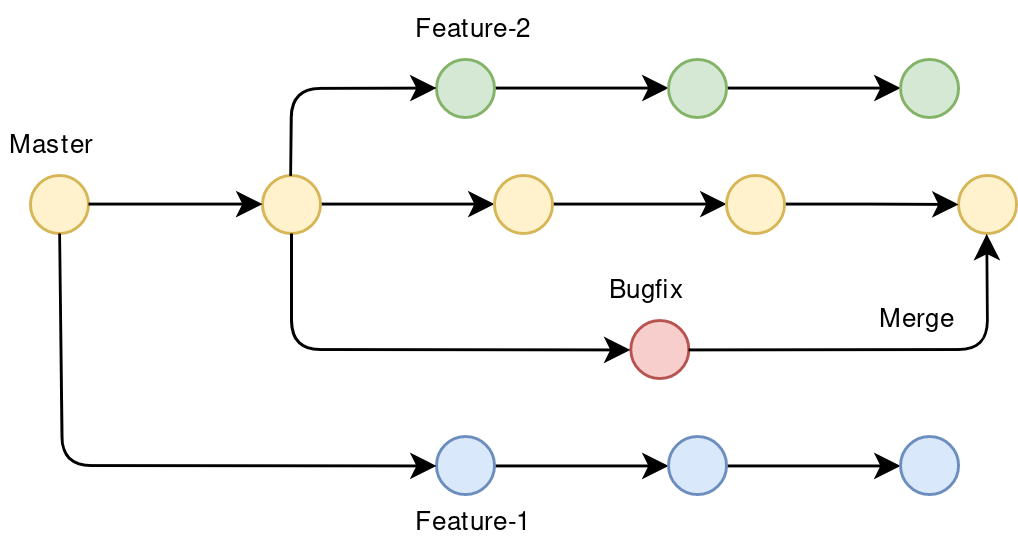
\includegraphics[scale=0.25]{./gfx/git-history-branch.png}
    \centering
    \caption{Eine beispielhafte Darstellung einer möglichen \emph{History} in Git.}\label{fig:git-history}
\end{figure}

Wenn man sich nun jedoch einen solchen \emph{Commit} genauer anschaut, fallen einige sehr interessante Details auf.
In Listing~\ref{lst:raw-commit} kann die Struktur einer solchen Datei gesehen werden und es sind mehrere direkte Identifikatoren und Metadaten zu sehen.
Zum einen ist der volle Name und die Email Adresse ersichtlich, welche vermutlich zu einer vollständigen Identifikation ausreichen würden.
Zudem ist Timestamp mit dem momentanen UTC Offset des Erstellers des \emph{Commits} eingebunden.

\begin{minted}[linenos]{text}
    tree      cd7d001b696db430b898b75c633686067e6f0b76
    parent    c19b969705e5eae0ccca2cde1d8a98be1a1eab4d
    author    Arne Beer <test@eintest.de> 1513434723 +0100
    committer Arne Beer <test@eintest.de> 1513434723 +0100

    Chapter 2, acronyms
\end{minted}
\begingroup
\captionof{listing}{Eine Git \emph{Commit} Datei. Auf unterster Ebene wird ein \emph{Commit} nur durch eine Textdatei in diesem Format dargestellt.\label{lst:raw-commit}}
\endgroup

Es ist folglich für jede neue Version zu sehen, wer diese erstellt hat, wann er sie erstellt hat und in welcher Zeitzone sich diese Person zu diesem Zeitpunkt aufgehalten hat.
Ebenfalls verbunden mit einem Commit sind alle Änderungen, die der Autor zwischen dieser und der letzten Version vorgenommen hat.


\subsection{GitHub}
GitHub ist die zur Zeit größte Open-Source Plattform mit über 96 Millionen öffentlichen Repositories.
Es ist eine Seite, die zur Verbreitung von Wissen, öffentlicher Software, zum Lernen sowie zum entwickeln kommerzieller Projekte verwendet wird.
Neben dem bloßen Bereitstellen einer Plattform, werden zudem Tools angeboten, welche die Kollaboration zwischen Entwicklern vereinfacht.
Dadurch wird die Hürde zum Beitragen an fremden Projekten deutlich gesenkt und dementsprechend sogar Kollaboration gefördert.




\section{Zusammenfassung}

\section{Literatur}

\printbibliography
\end{document}
